本章では Icarus Verilog/NC-Verilog/VCS での論理シュミレーションの実行時間と
ArchHDL での実行時間を比較し,評価する.

Icarus Verilog/ArchHDL の実行環境は OS が Ubuntu12.04,カーネルが 64ビットの
Linux 3.2.0-39-generic, CPU は
Intel Core i7-3770K CPU @ 3.50GHz,メモリーは
$16\,\mathrm{GB}$ である.

NC-Verilog/VCS の実行環境は OS が CentOS5.9,カーネルが 64ビットの
Linux 2.6.18-348.4.1.el5, CPU は
hogehoge,メモリーは
$16\,\mathrm{GB}$ である.


## ステンシル計算回路による評価

\if0
\begin{table}[t]
 \caption{ステンシル計算回路でのプロファイリング結果 1.1}
 \label{table:stencil_prof1.1}
 \begin{center}
  % \setlength{\tabcolsep}{3pt}
  \begin{tabular}{lr} \toprule
  関数名 & 実行時間に占める割合 (\%) \\ \midrule
  reg::Update() (合計) & 16.57 \\
  ArchHDL::Step() & 12.47 \\
  brk & 15.05 \\ \bottomrule
  \end{tabular}
 \end{center}
\end{table}
\fi


\begin{figure}[t]
 \centering
 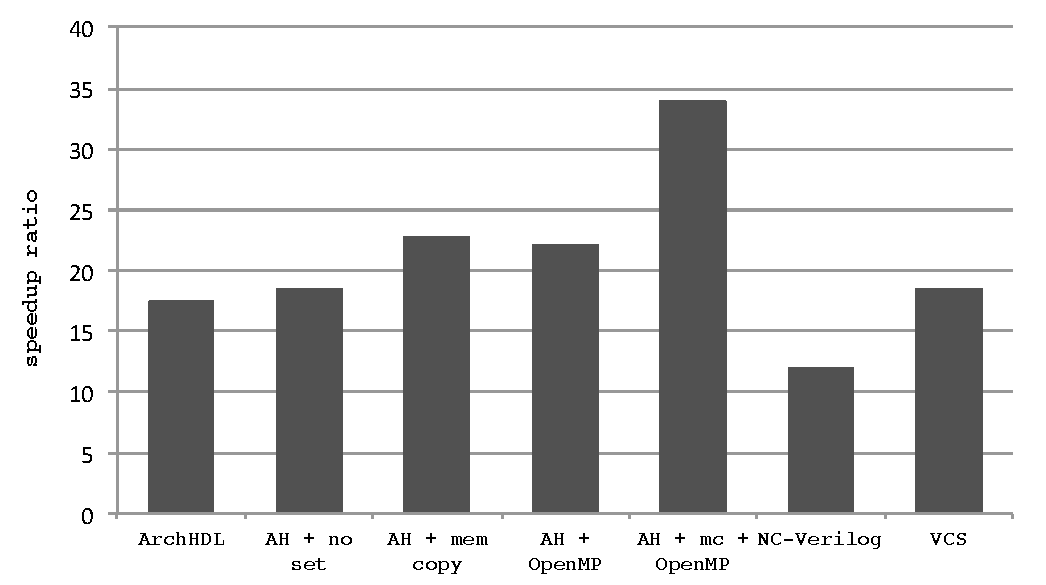
\includegraphics[clip,width=\linewidth]{stencil}
 \caption{ステンシル計算回路の Icarus Verilog と比較した実行時間の速度向上比}
 \label{fig:stencil}
\end{figure}

\figref{fig:stencil} はステンシル計算回路での実行結果である.

縦軸は Icarus Verilog と比較したそれぞれの速度向上比である.

OpenMP による並列化はスレッド数を 8 個にして計測している.

ステンシル計算回路の場合は Update() は 325,469,175 回呼ばれているのに対して,
reg の値が更新されるのは 320,323,415 回であり,
reg の値に更新がないのは 5,145,760 回である.つまり更新がないのは全体の約
$1.58\%$ 程度に過ぎない.そのため set_ 変数なしの方が高速になる.

また Update() は 325,469,175 回呼ばれているのでこのメソッド呼び出しを減らし,かつ代入をメモリーコピーにする v2.0 の効果は強力であるといえる.

また Module が 133 個,reg が 991 個存在する回路なので並列化の効果も大きい.

NC-Verilog は ArchHDL より高速でない.VCS は ArchHDL と set_ 変数なしの実装より高速であるが,メモリーコピーにする実装よりは高速でない.また並列化を行ったものより高速でない.


## マイクロベンチマークによる評価

カウンター回路を $n$ 回試行するもの.

(現状カウンター回路は NC-Verilog だけ一定でそれ以外線形なので見せ方工夫いる)

$n$ 個のカウンター回路を実行するもの.

(一定数超えると並列化の効果が出てくる)


\begin{figure}[t]
 \centering
 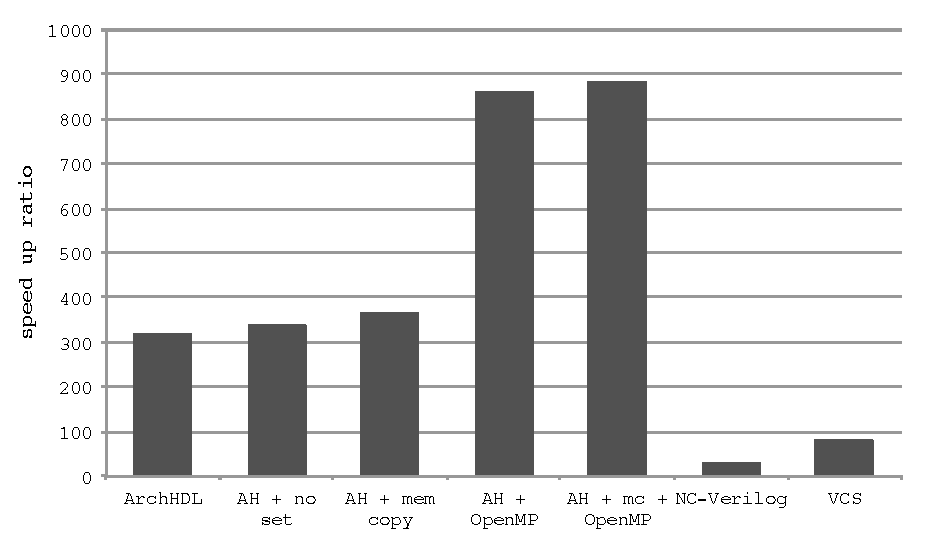
\includegraphics[clip,width=\linewidth]{xorshift}
 \caption{XORSHIFT による乱数生成器の Icarus Verilog と比較した実行時間の速度向上比}
 \label{fig:xorshift}
\end{figure}

\figref{fig:xorshift} は XORSHIFT による乱数生成器での実行結果である.試行回数は 16,777,216 回である.

縦軸は Icarus Verilog と比較したそれぞれの速度向上比である.









## 高速化の解析







